\section{Results: Final Objective Values and Convergence}

\subsection{Final Objective Values}
\autoref{fig:final_distributions} compares the final objective values across ten runs, and \autoref{tab:results} summarizes the same distributions using medians and interquartile ranges. Lower values are better. The plain EDA obtains the lowest median on all four benchmarks. Its advantage is largest on Sphere, where the median is $3.55\times10^{-5}$, compared with $3.12\times10^{-4}$ for BO and $5.02\times10^{-4}$ for L-BFGS-B. On Ackley, its median is $0.0897$, compared with $0.417$ and $0.484$ for the classical and BO hybrids, respectively.

The distributions overlap more on Rastrigin and Rosenbrock. On Rastrigin, the medians are $6.44$ for the plain EDA, $7.44$ for BO, and $8.11$ for L-BFGS-B; on Rosenbrock, they are $4.61$, $5.49$, and $7.16$, respectively. BO therefore achieves a lower median final objective value than the classical hybrid on three benchmarks, with Ackley as the exception, but neither hybrid improves on the plain EDA by this measure. The spread of the individual points shows that the ranking can differ between runs.

\begin{table}[H]
\caption{Final objective after 600 evaluations. Each entry gives the median, with the interquartile range below. The lowest median per benchmark is bold.}
\label{tab:results}
\centering
\small
\setlength{\tabcolsep}{5pt}
\begin{tabular}{lrrr}
\toprule
Benchmark & Plain EDA & EDA + L-BFGS-B & EDA + BO \\
\midrule
Sphere & $\mathbf{3.55\!\times\!10^{-5}}$ & $5.02\!\times\!10^{-4}$ & $3.12\!\times\!10^{-4}$ \\
 & $[9.68\!\times\!10^{-6},7.38\!\times\!10^{-5}]$ & $[3.81\!\times\!10^{-4},6.17\!\times\!10^{-4}]$ & $[2.36\!\times\!10^{-4},6.45\!\times\!10^{-4}]$ \\[3pt]
Rastrigin & $\mathbf{6.44}$ & $8.11$ & $7.44$ \\
 & $[4.81,9.2]$ & $[7.17,11.4]$ & $[5.64,8.8]$ \\[3pt]
Ackley & $\mathbf{0.0897}$ & $0.417$ & $0.484$ \\
 & $[0.0486,0.0999]$ & $[0.253,0.804]$ & $[0.388,0.525]$ \\[3pt]
Rosenbrock & $\mathbf{4.61}$ & $7.16$ & $5.49$ \\
 & $[3.44,6.01]$ & $[3.82,9.74]$ & $[3.56,6.83]$ \\[3pt]
\bottomrule
\end{tabular}

\end{table}

\begin{figure}[H]
\centering
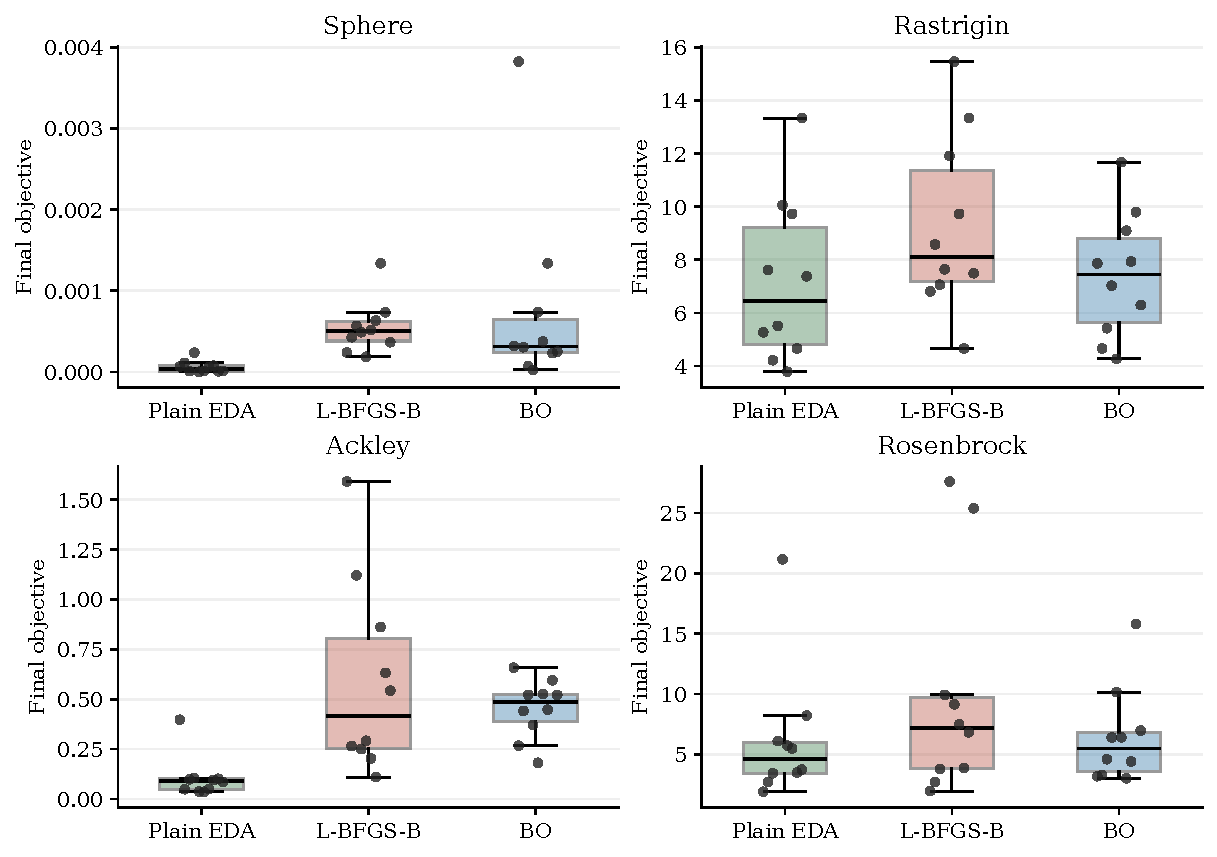
\includegraphics[width=\textwidth]{final_distributions.pdf}
\caption{Final objective values after 600 evaluations across ten seeds. Boxes show the interquartile range and median; points show all runs. Each benchmark uses its own linear vertical scale. Whiskers extend to the most extreme values within 1.5 interquartile ranges of the box.}
\label{fig:final_distributions}
\end{figure}

\subsection{Convergence}
\autoref{fig:convergence} shows the evolution of the best objective found. The horizontal axis counts all objective evaluations, including those used by LS. This makes the three methods comparable despite their different numbers of EDA generations. Each curve is the mean across ten runs, and the shaded band is the interquartile range.

\begin{figure}[H]
\centering
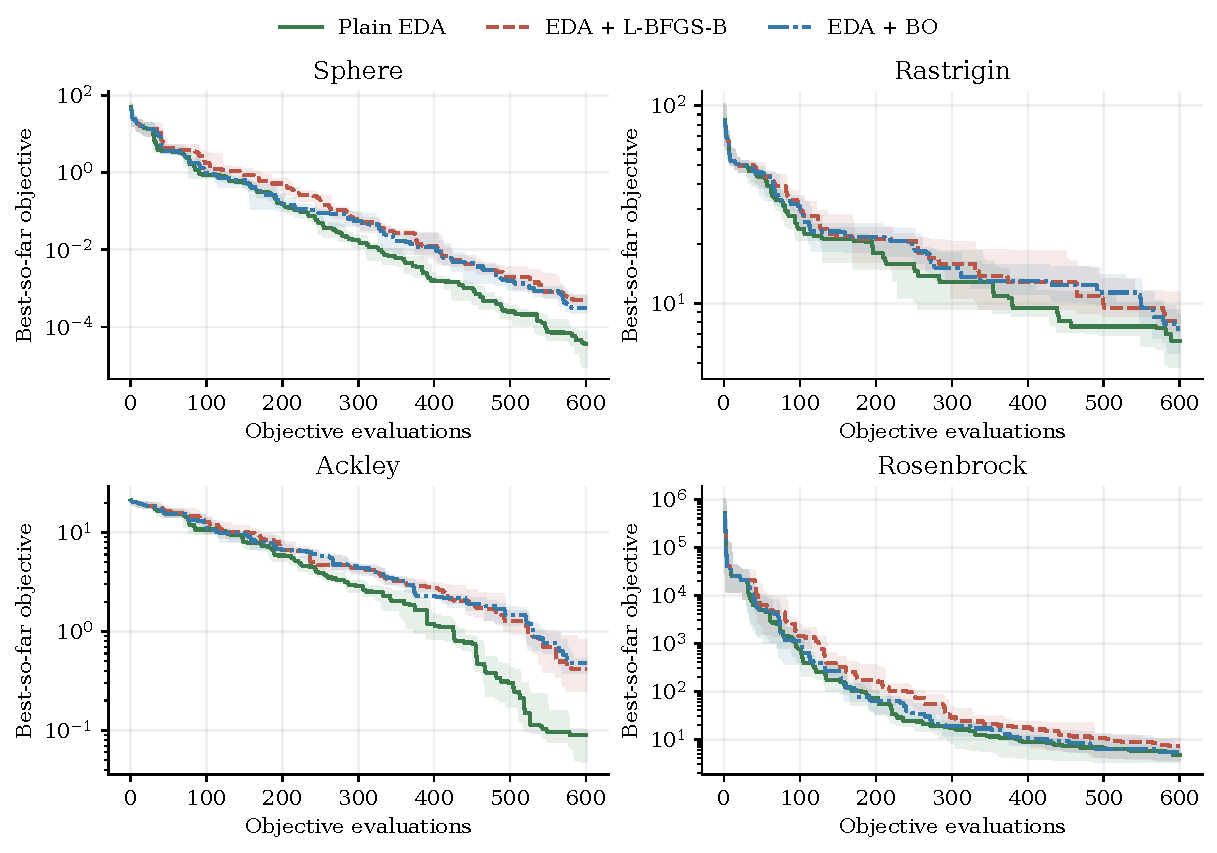
\includegraphics[width=\textwidth]{main_convergence.pdf}
\caption{Best-so-far objective over 600 evaluations. Lines show means and bands show interquartile ranges across ten seeds. Each panel uses its own logarithmic vertical scale.}
\label{fig:convergence}
\end{figure}

All three methods reduce the objective during the run, but the LS variants do not produce a better mean endpoint. On Sphere, the plain EDA finishes about one order of magnitude below the hybrids. On Rastrigin, the mean evaluation at which each run first finds its final best value is 505 for the plain EDA, 536 for L-BFGS-B, and 538 for BO. This leaves a longer final period without improvement than on the other benchmarks. On Sphere, Ackley, and Rosenbrock, the corresponding mean evaluations range from 571.5 to 594, so improvements are still found near the end of the budget.

No run reaches an objective value of $10^{-6}$ or lower. The observed plateaus therefore indicate a lack of further improvement within the available budget, rather than convergence to the global optimum. Under these settings, using all evaluations for population search gives the best mean final performance. Local refinement can improve the selected individual, but its evaluation cost does not translate into a better overall mean result in these experiments.
